

In the proposed architecture, the \textit{Smart Gateway} is the central module of the system, connecting the \textit{SmartBoxes} to the \acs{HIS}. It is responsible for the management of devices and their associations -- \textit{SmartBox} to \textit{Biosticker} and \textit{SmartBox} to user -- managing, maintaining and storing the data that is generated by these, as well as handling any communication to and from the \acs{HIS}. 


\paragraph{} Regarding the hardware platform used to implement the \textit{Smart Gateway}, in context of the \acs{WoW} project, we use the Intel NUC NUC8i7BEH\footnote{\url{https://ark.intel.com/content/www/br/pt/ark/products/126140/intel-nuc-kit-nuc8i7beh.html}}.

\begin{figure}[H]
    \centering
    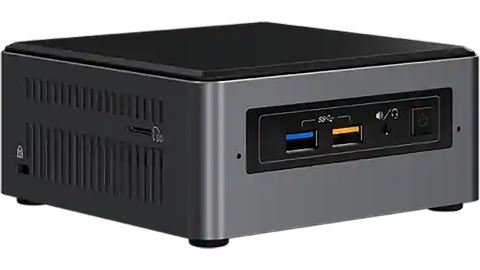
\includegraphics[width=0.5\linewidth]{images/gateway-image.png}
    \caption[Intel NUC NUC8i7BEH.]{Intel NUC NUC8i7BEH.}
    \label{fig:gateway_image}
\end{figure}


\paragraph{} In the next sections, we propose a service architecture for the \textit{Smart Gateway} in order to fulfill the aforementioned features.

% The \textit{Smart Gateway} maintains a list of all the \textit{SmartBoxes} that are managed by the system, as well as every \textit{Biosticker} and every sensor in the \textit{Biosticker} (which are used to indicate respective biosignal to the \acs{HIS}). 


\section{Service Architecture}

The \textit{Smart Gateway} must 

\paragraph{} Figure \ref{fig:gateway_serviceoverview} illustrate the different services implemented in the \textit{Smart Gateway}

\begin{figure}[H]
    \centering
    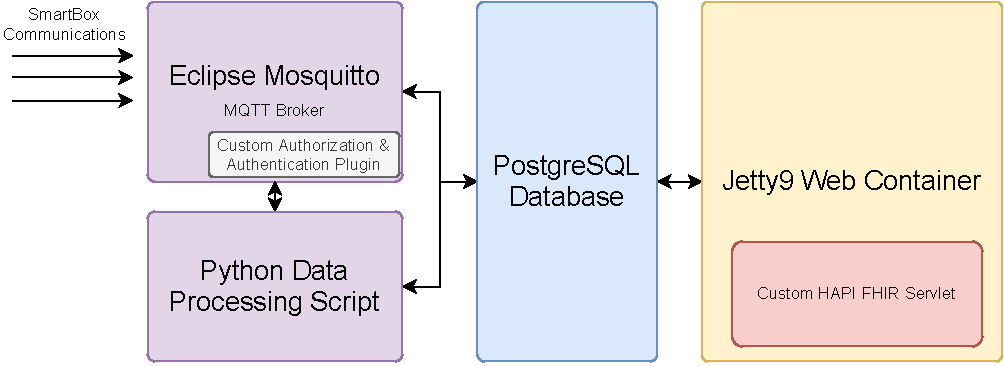
\includegraphics[width=\linewidth]{images/service overview gateway.pdf}
    \caption[Service architecture implemented in the \textit{Smart Gateway}.]{Service architecture implemented in the \textit{Smart Gateway}. The diagram displays the different technologies used throughout the development. The services communicate with each other using Unix Sockets, a Linux exclusive protocol for \acf{IPC}.}
    \label{fig:gateway_serviceoverview}
\end{figure}


\subsection{Security on Linux}
- o isolamento dos processos é feito através do "utilizador" que está a executar o processo. cada processo tem apenas acesso aos seus serviços.

- indicar que estamos a usar Unix Sockets para a comunicação entre processos;

- o uso de unix sockets permite usar o sistema de permissões do sistema operativo para controlar o acesso às sockets (através dos ``utilizadores'' que estão a executar os serviços).

\paragraph{} As seen above, these services have 

\section{Data Storage}

The data storage in the \textit{Smart Gateway} is one of the most important components of the device, as it holds the information used by all services in the \textit{Smart Gateway}. Given the importance of this component, it is crucial to use a solution which offers reliability above all with great performance for our use case.  

\paragraph{} As discussed in Section \ref{sec:iot-model-layer4}, No\acs{SQL} databases are appealing for \acs{IoT} applications, since these have great performance..

% it is important to choose a solution which offers availability

% PostgreSQL offers a balance between \footnote{\url{https://itnext.io/benchmark-databases-in-docker-mysql-postgresql-sql-server-7b129368eed7?gi=a506815fb197}}

\subsection{Database Schema}
Figure \ref{fig:wow-dbschema-full} contains the database model implemented in our PostgreSQL database. It describes all information that is contained in the \textit{Smart Gateway}, the relations within that data, organized according to the functionality it is related to, which will be explored in greater detail in the next sections.


\begin{figure}[H]
    \centering
    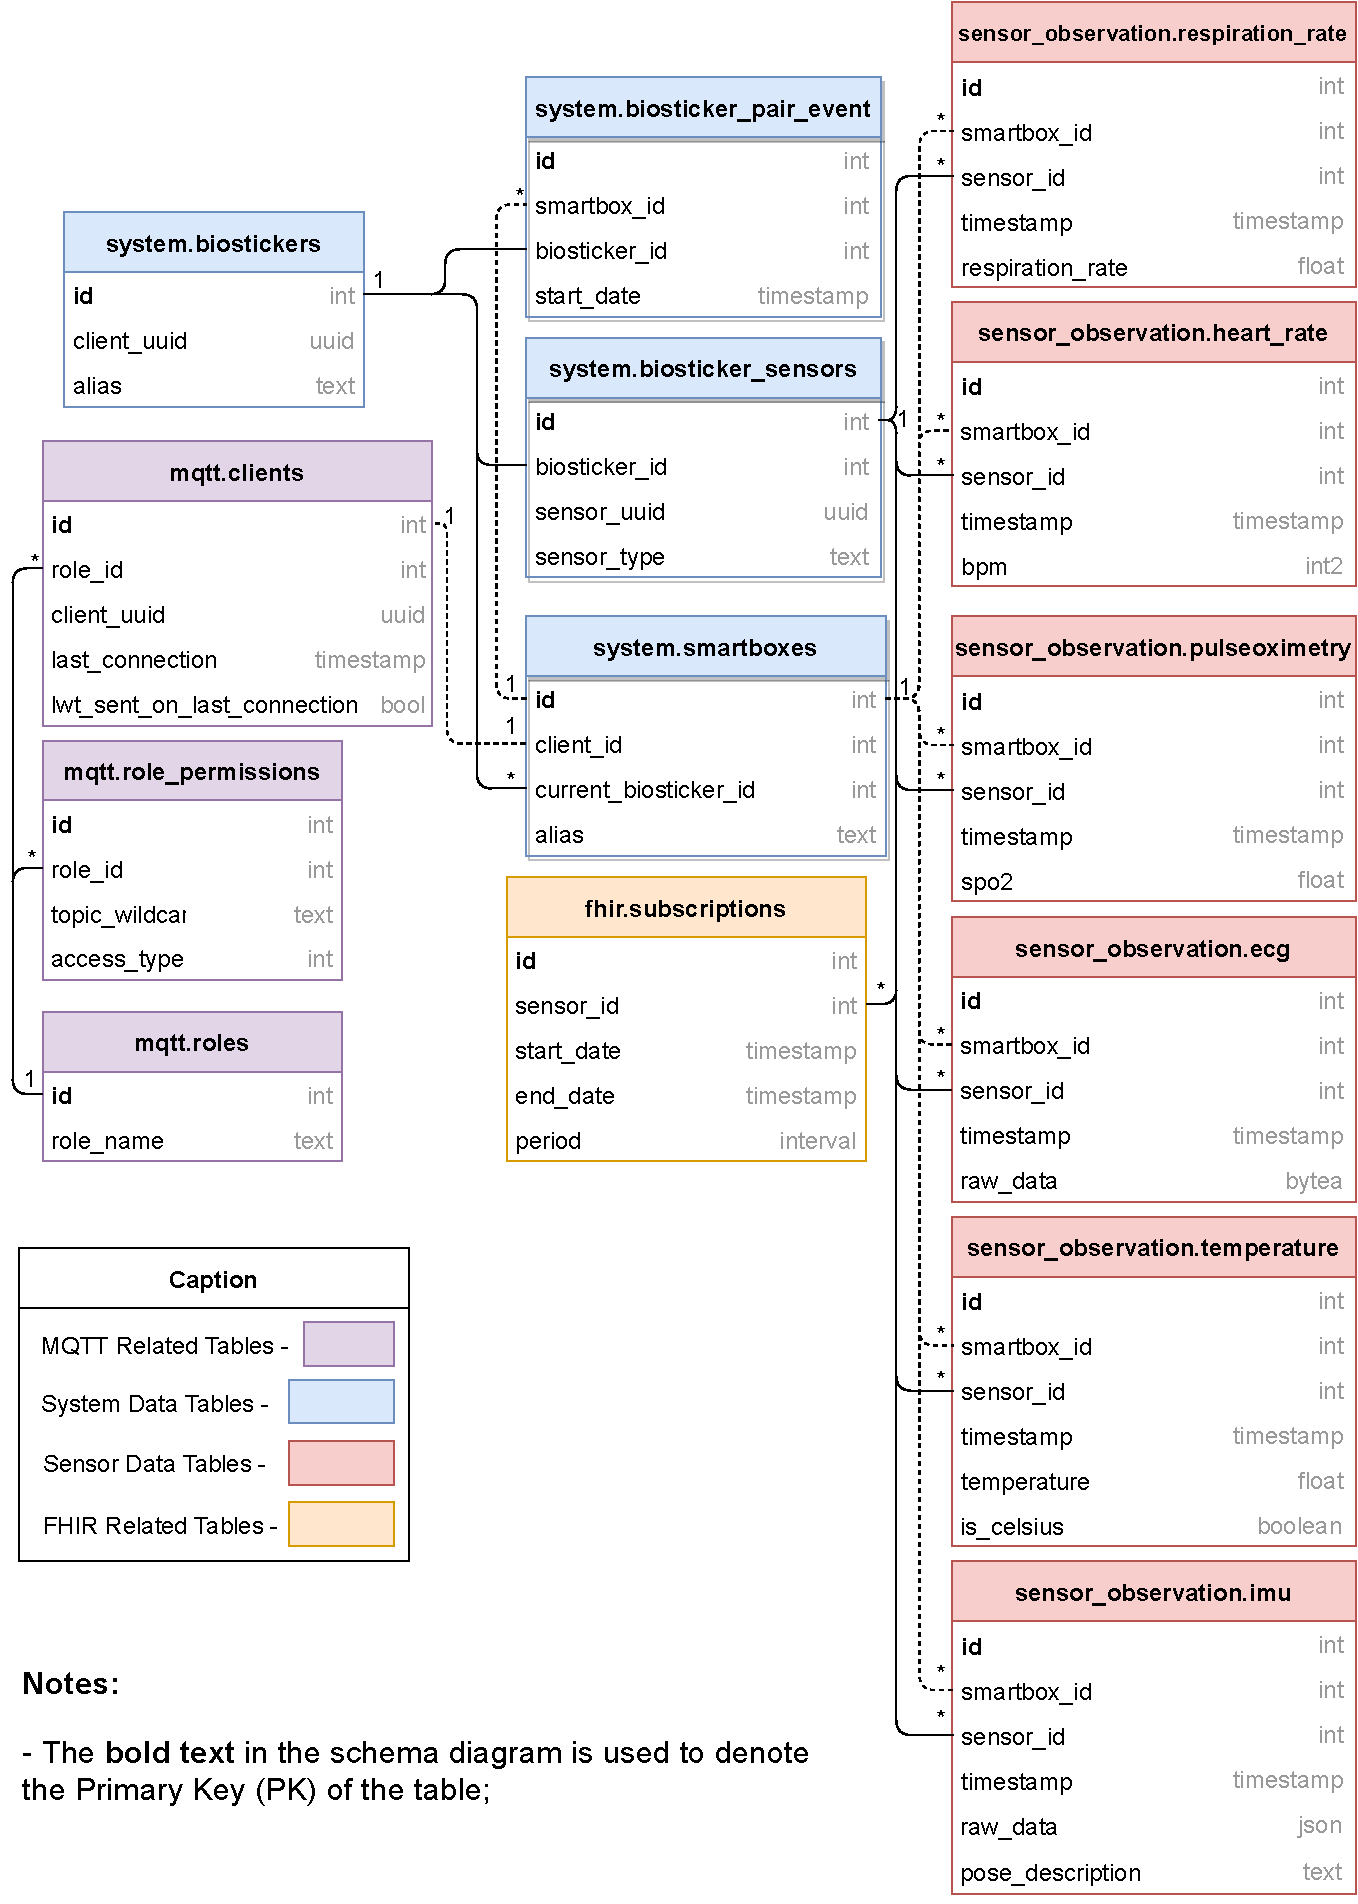
\includegraphics[width=0.86\linewidth]{images/database-schema-general.pdf}
    \caption[Database schema implemented in the \textit{Smart Gateway}.]{Database schema implemented in the \textit{Smart Gateway}.}
    \label{fig:wow-dbschema-full}
\end{figure}

\subsubsection{MQTT Client Information}

Figure \ref{fig:wow-dbschema-mqtt} contains the information relevant for \acs{MQTT} communications, mostly related with security. In order to ensure that each device only has access to its own resources, the system implements a \acf{RBAC} policy. 
In this type of access control, the system allows and revokes access to resources according to the role of the device.

\paragraph{} In context of the \acs{WoW} project, the following roles are used:

\begin{itemize}
    \item \textit{SmartBox} role: Indicates the \acs{MQTT} client is a \textit{SmartBox}.
    \item ``Pyservice'' role: Indicates the \acs{MQTT} client is actually the data processing service, also contained in the \textit{Smart Gateway}.
    \item Developer device role: Indicates the \acs{MQTT} client is a developer device, used solely for debugging purposes.
\end{itemize}

\begin{figure}[H]
    \centering
    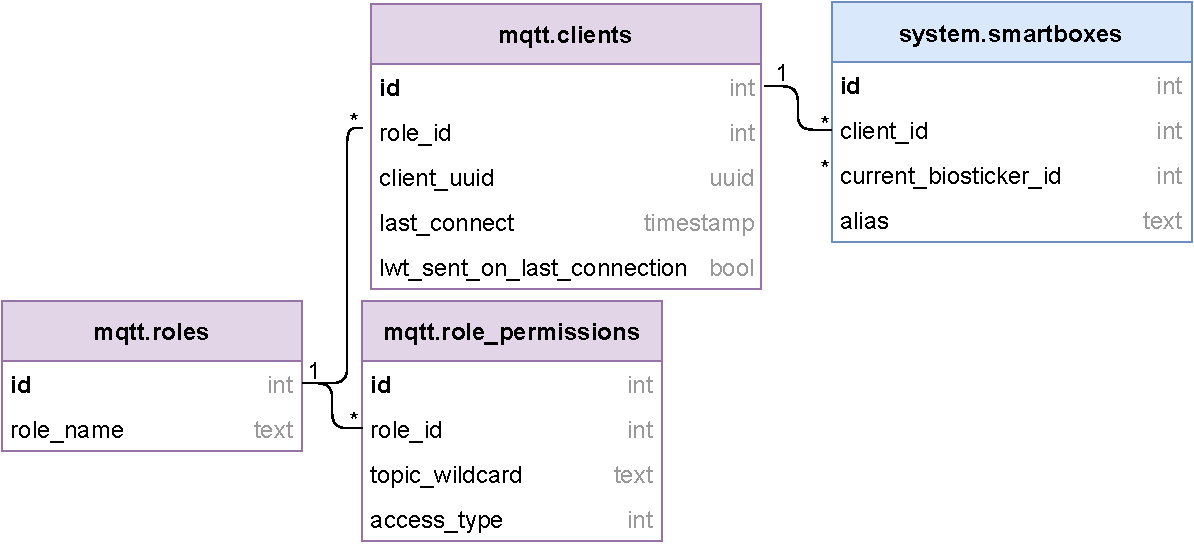
\includegraphics[width=\linewidth]{images/database-schema-mqtt.pdf}
    \caption[\acs{MQTT} information in the schema implemented in the \textit{Smart Gateway}.]{\acs{MQTT} information in the schema implemented in the \textit{Smart Gateway}.}
    \label{fig:wow-dbschema-mqtt}
\end{figure}

\subsubsection{Sensor Data}
\dots 

\begin{figure}[H]
    \centering
    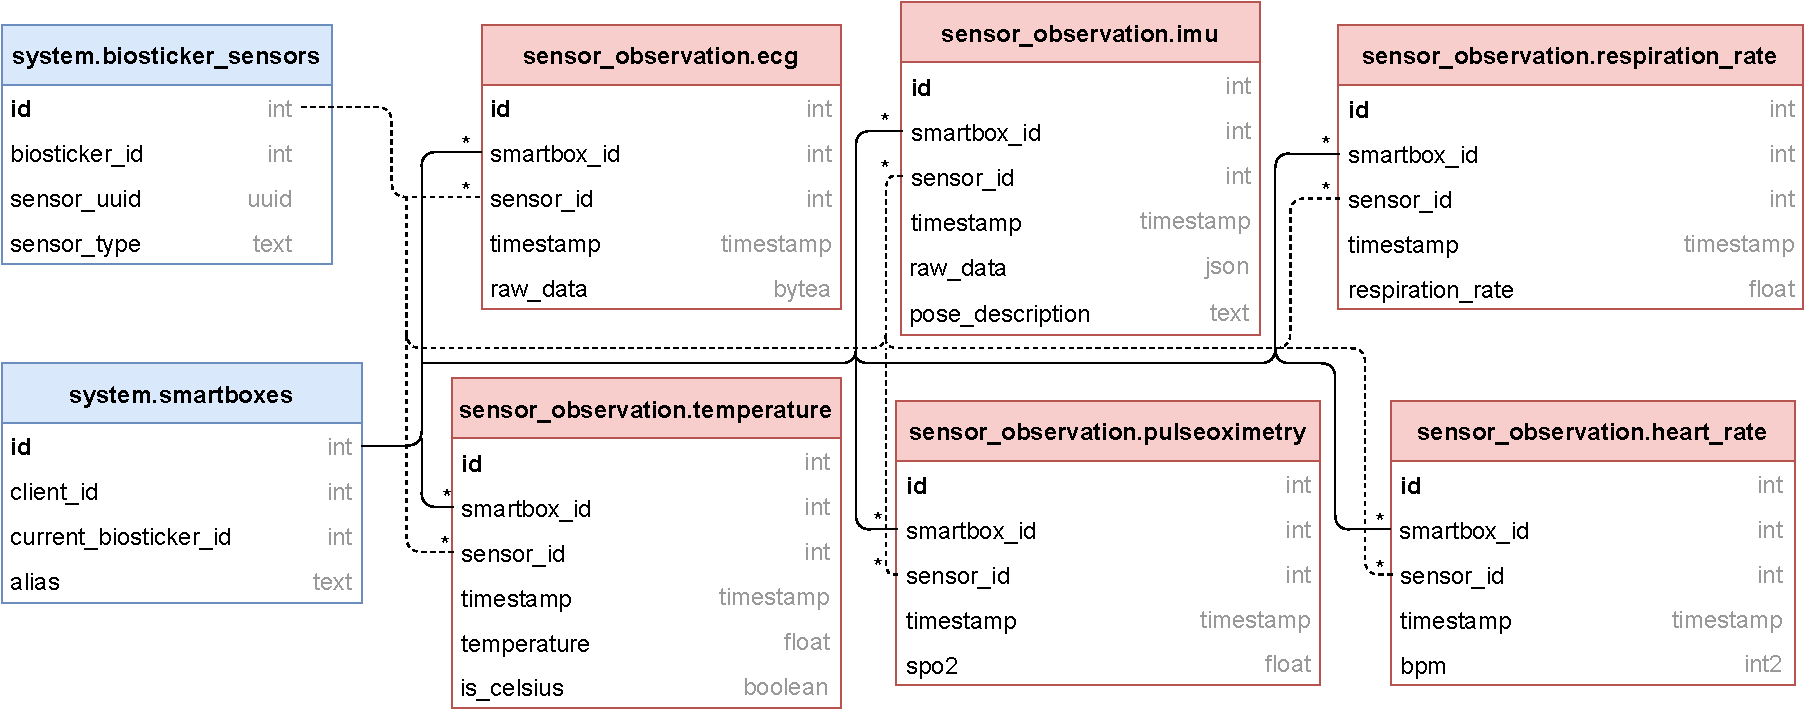
\includegraphics[width=\linewidth]{images/database-schema-sensordata.pdf}
    \caption[test]{test}
    \label{fig:wow-dbschema-sensors}
\end{figure}

\subsubsection{FHIR Related Information}
\dots 

\begin{figure}[H]
    \centering
    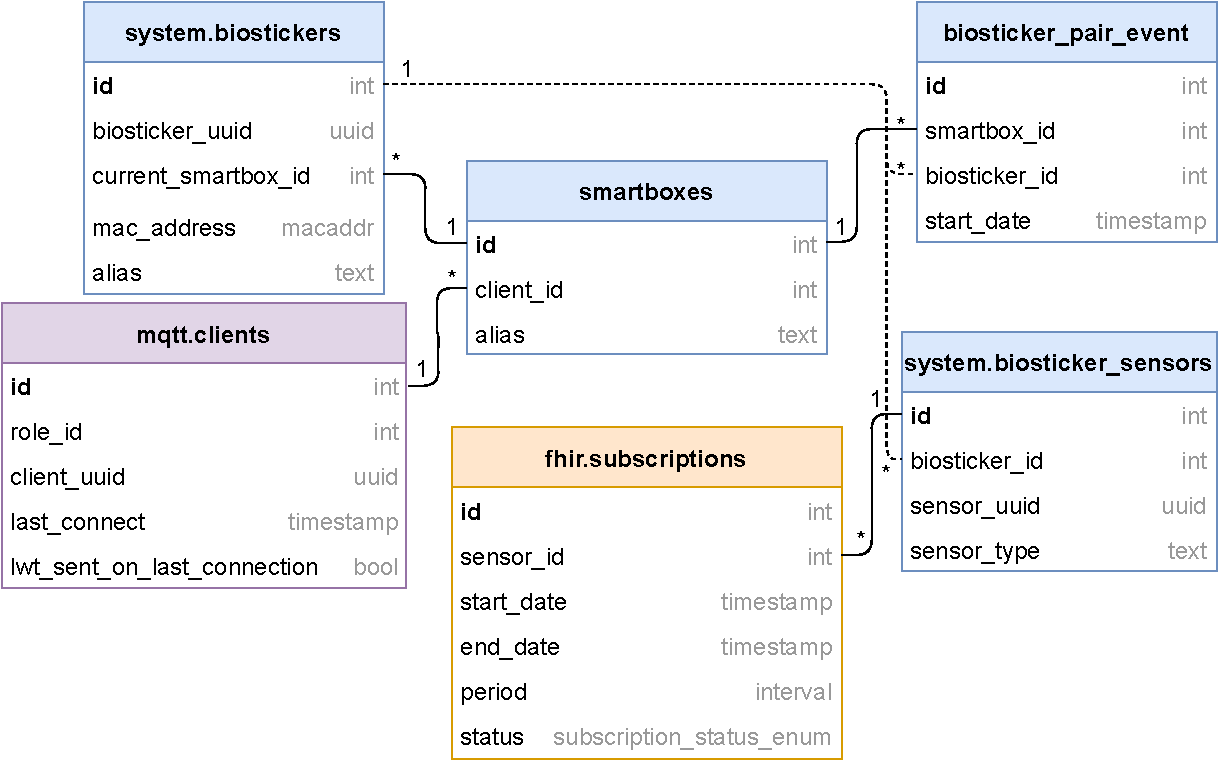
\includegraphics[width=\linewidth]{images/database-schema-fhir.pdf}
    \caption[test]{test}
    \label{fig:wow-dbschema-fhir}
\end{figure}


\subsubsection{Stored Procedures}

%During development, we noticed that our database service was consuming a concerning amount of resources when 
- de modo a maximizar o desempenho do serviço da base de dados, os diferentes pedidos de base de dados (queries) foram configurados e pré-compilados na base de dados. isto reduz o tamanho dos pedidos enviados à base de dados (pois em vez de enviar transações complexas, executamos apenas uma função na base de dados), faz com que a base de dados não tenha de validar a estrutura dos pedidos (porque já foi pre-compilada), particularmente para eviar injeções de SQL.

\section{Connection to the SmartBoxes}

As previously mentioned, the connection to the \textit{SmartBoxes} is performed via \acs{MQTT}. \acs{MQTT} is a centralized protocol, in which the clients (\textit{SmartBoxes}) connect to a broker, which acts as a middle-man for the communication, managing the requests from all clients accordingly. In our system, the broker is contained within the \textit{Smart Gateway}, and is the service responsible for ensuring the communication between the \textit{SmartBoxes} and our \acs{IoT} system.

\paragraph{} To implement this \acs{MQTT} broker, we use the open-source Eclipse Mosquitto\footnote{Eclipse Mosquitto -- An open-source \acs{MQTT} broker: \url{https://mosquitto.org/}}. Mosquitto is a lightweight \acs{MQTT} broker that supports the \acs{MQTT} protocol versions 5.0, 3.1.1 and 3.1 and is widely used by the community, making it a fitting solution for the \acs{WoW} project.

\paragraph{} One of the 



It is extremely flexible since it allows developers to extend its functionality using plugins

exposes an \acs{API}

extensible 

\paragraph{} 


\subsection{Specification for \acs{MQTT} Communication}
- indicar que foi proposta uma especificação para a comunicação MQTT

\subsection{Authorization and Authentication Plugin}
- 
- a segurança no MQTT é feita através de 2 points
- a segurança no mosquitto atualmente é feita através de um ficheiro estático (lol) que define as permissões dos clientes que acedem o servidor.
- de modo a assegurar 

\section{Integration with GlobalCare}

- Mini introdução ao FHIR;
- mencionar camada de interoperabilidade da globalcare;
- indicar que optou-se usar HAPI devido ao facto de ser uma iniciativa open-source suportada por uma empresa de software hospitalar de renome.
- HAPI FHIR é baseada em Java servlets, fazer mini introdução do que são servlets e explicar o porquê de usar Jetty para correr servlets (é um web container, cujo objetivo é correr servlets). 

\subsection{FHIR Server}

- Falar do que são os FHIR Resources, e mais especificamente dos Resources usados para transmitir os dados -> Bundle, Device, Observation
- Apresentação do diagrama de comunicação de informação

\section{Summary}

In this chapter, we presented the different components which form the \textit{Smart Gateway}.